\documentclass[
  bibliography=totoc,     % Literatur im Inhaltsverzeichnis
  captions=tableheading,  % Tabellenüberschriften
  titlepage=firstiscover, % Titelseite ist Deckblatt
]{scrartcl}

% Paket float verbessern
\usepackage{scrhack}

% Warnung, falls nochmal kompiliert werden muss
\usepackage[aux]{rerunfilecheck}

% unverzichtbare Mathe-Befehle
\usepackage{amsmath}
% viele Mathe-Symbole
\usepackage{amssymb}
% Erweiterungen für amsmath
\usepackage{mathtools}

% Fonteinstellungen
\usepackage{fontspec}
% Latin Modern Fonts werden automatisch geladen
% Alternativ:
%\setromanfont{Libertinus Serif}
%\setsansfont{Libertinus Sans}
%\setmonofont{Libertinus Mono}
\recalctypearea % Wenn man andere Schriftarten gesetzt hat,
% sollte man das Seiten-Layout neu berechnen lassen

% deutsche Spracheinstellungen
\usepackage{polyglossia}
\setmainlanguage{german}


\usepackage[
  math-style=ISO,    % ┐
  bold-style=ISO,    % │
  sans-style=italic, % │ ISO-Standard folgen
  nabla=upright,     % │
  partial=upright,   % ┘
  warnings-off={           % ┐
    mathtools-colon,       % │ unnötige Warnungen ausschalten
    mathtools-overbracket, % │
},                       % ┘
]{unicode-math}

% traditionelle Fonts für Mathematik
\setmathfont{Latin Modern Math}
% Alternativ:
%\setmathfont{Libertinus Math}

\setmathfont{XITS Math}[range={scr, bfscr}]
\setmathfont{XITS Math}[range={cal, bfcal}, StylisticSet=1]

% Zahlen und Einheiten
\usepackage[
locale=DE,                   % deutsche Einstellungen
separate-uncertainty=true,   % immer Fehler mit \pm
per-mode=symbol-or-fraction, % / in inline math, fraction in display math
]{siunitx}

% chemische Formeln
\usepackage[
version=4,
math-greek=default, % ┐ mit unicode-math zusammenarbeiten
text-greek=default, % ┘
]{mhchem}

% richtige Anführungszeichen
\usepackage[autostyle]{csquotes}

% schöne Brüche im Text
\usepackage{xfrac}

% Standardplatzierung für Floats einstellen
\usepackage{float}
\floatplacement{figure}{htbp}
\floatplacement{table}{htbp}

% Floats innerhalb einer Section halten
\usepackage[
section, % Floats innerhalb der Section halten
below,   % unterhalb der Section aber auf der selben Seite ist ok
]{placeins}

% Seite drehen für breite Tabellen: landscape Umgebung
\usepackage{pdflscape}

% Captions schöner machen.
\usepackage[
  labelfont=bf,        % Tabelle x: Abbildung y: ist jetzt fett
  font=small,          % Schrift etwas kleiner als Dokument
  width=0.9\textwidth, % maximale Breite einer Caption schmaler
]{caption}
% subfigure, subtable, subref
\usepackage{subcaption}

% Grafiken können eingebunden werden
\usepackage{graphicx}
% größere Variation von Dateinamen möglich
\usepackage{grffile}

% schöne Tabellen
\usepackage{booktabs}

% Verbesserungen am Schriftbild
\usepackage{microtype}

% Literaturverzeichnis
\usepackage[style=alphabetic,]{biblatex}
% Quellendatenbank
\addbibresource{lit.bib}
\addbibresource{programme.bib}

% Hyperlinks im Dokument
\usepackage[
  unicode,        % Unicode in PDF-Attributen erlauben
  pdfusetitle,    % Titel, Autoren und Datum als PDF-Attribute
  pdfcreator={},  % ┐ PDF-Attribute säubern
  pdfproducer={}, % ┘
]{hyperref}
% erweiterte Bookmarks im PDF
\usepackage{bookmark}

% Trennung von Wörtern mit Strichen
\usepackage[shortcuts]{extdash}

\title{V64: Moderne Interferometrie}
\author{
  Simon Schulte
  \texorpdfstring{
    \\
    \href{mailto:simon.schulte@udo.edu}{simon.schulte@udo.edu}
  }{}
  \texorpdfstring{\and}{, }
  Tim Sedlaczek
  \texorpdfstring{
    \\
    \href{mailto:tim.sedlaczek@udo.edu}{tim.sedlaczek@udo.edu}
  }{}
}
\publishers{TU Dortmund – Fakultät Physik}

\date{Durchführung: 13.06.2018\\
      Abgabe: 04.07.2018}


\begin{document}

\maketitle
\thispagestyle{empty}
\setcounter{page}{1}
\pagenumbering{arabic}

\section{Theorie}
\label{sec:theorie}
Bei diesem Versuch sollen mittels Interferometrie die Brechungsindizes von Glas
und Luft bestimmt werden. Dazu wird in diesem Fall ein Sagnac-Interferometer
verwendet, welches sich baulich von einem Michelson-Interferometer vor allem
dadurch unterscheidet, dass beide Strahlen ungefähr den gleichen Strahlengang
durchqueren und damit äußere Einflüsse zu kleineren Abweichungen führen.

\subsection{Funktionsweise des Sagnac-Interferometers}
\label{sub:funktionsweise}
Bei dem Sagnac-Interferometer wird ein Laserstrahl, der von einem Helium-Neon-Laser
erzeugt wird, über zwei Spiegel auf einen so genannten PBSC gelenkt.
PBSC steht für Polarizing-Beam-Splitter-Cube. Er wirkt dabei, wie der
halbdurchlässige Spiegel in einem Michelson-Interferometer, als Strahlteiler.
Hierzu besteht er aus zwei Prismen, die über ein Dielektrikum verbunden sind.
Das Dielektrikum sorgt dafür, dass der transmittierte Strahl dem P-polarisierten
Anteil des einfallenden Strahls entspricht und der reflektierte Strahl dem
S-polarisierten Anteil. Die beiden Strahlen durchlaufen anschließend die, durch
drei weitere Spiegel geformte, Bahn in entgegengesetzter Richtung und treffen dann
an dem PBSC wieder aufeinander. Da sie senkrecht aufeinander liegende Polarisationsrichtungen
besitzen interferieren sie an dieser Stelle noch nicht. Hierzu befindet sich im weiteren
Strahlengang ein zweiter PBSC, welcher um $\SI{45}{\degree}$ gekippt ist. Durch
den Winkel besitzen beide Strahlen in der Ebene des PBSC eine senkrechte und
eine parallele Komponente. Diese werden entsprechend aufgespalten und treffen als
zwei überlagerte Strahlen mit je einer gemeinsamen Polarisationsrichtung
auf zwei Photodioden.
Der Aufbau eines Sagnac-Interferometers ist in Abbildung \ref{fig:1} zu sehen.
\begin{figure}[H]
  \centering
  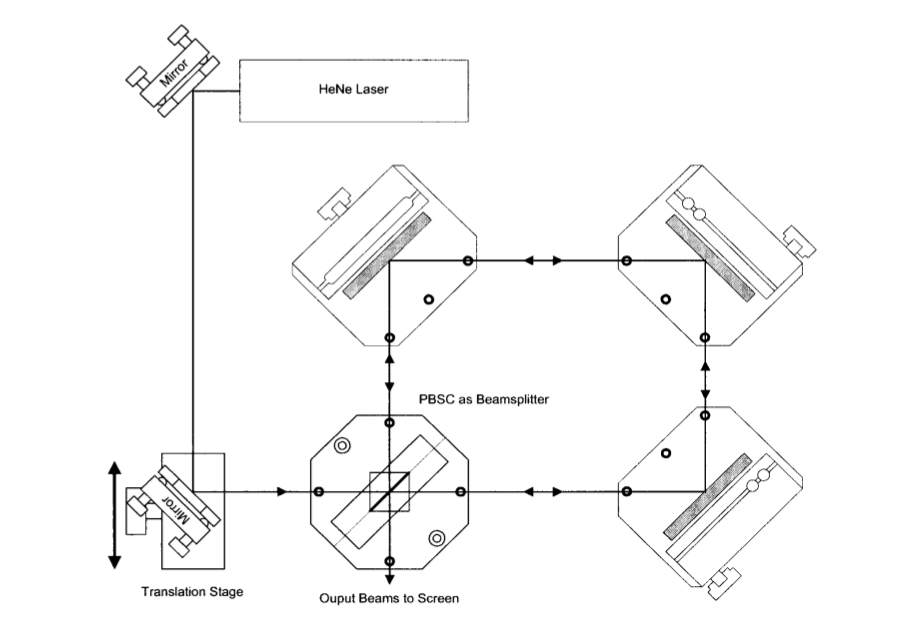
\includegraphics[width=0.7\textwidth]{Bild1.png}
  \caption{Aufbau eines Sagnac-Interferometers \cite{anleitung}.}
  \label{fig:1}
\end{figure}

\subsection{Kontrast}
\label{sub:kontrast}
Bei der Interferometrie ist es Sinnvoll bei maximalem Kontrast zu arbeiten.
Der Kontrast beschreibt dabei die Differenz der Intensität von Interferenzmaximum
und Minimum.
Dafür gilt:
\begin{equation}
  \mathup{K} = \frac{\mathup{I_\mathup{max}}-\mathup{I_\mathup{min}}}{\mathup{I_\mathup{max}}+\mathup{I_\mathup{min}}}.
  \label{eqn:kontrast}
\end{equation}
In dem Optimalfall ($\mathup{I_\mathup{min}} = 0$) ergibt sich also ein Kontrast
von 1.\\
Da bei dem Sagnac-Interferometer die stärke der Interferenz von der
Intensität der beiden Strahlen abhängt, die den ersten PBSC verlassen, wird die
Maximierung des Kontrastes über einen Polarisationsfilter vor dem ersten PBSC
vorgenommen. Um einen Zusammenhang zwischen Polarisationswinkel $\phi$ und Kontrast
zu erhalten wird zunächst das Verhalten der Intensität in Abhängigkeit von dem Winkel
untersucht.
Für die Intensität gilt:
\begin{equation}
  \mathup{I} \propto \bigl< \bigl| \mathup{E_1} \cos\left(\phi\right) \cos\left(\omega t\right) + \mathup{E_2} \sin\left(\phi\right) \cos\left(\omega t + \delta\right) \bigr| ^2 \bigr>.
  \label{eqn:intens}
\end{equation}
Dies ist ein zeitliche Mittelwert über eine Periode. $\mathup{E_1}$ und $\mathup{E_2}$
sind die elektrischen Feldstärken der beiden Lichtstrahlen, die den PBSC verlassen.
$\delta$ ist ein Phasenunterschied, der für konstruktive bzw. destruktive Interferenz
sorgt. Es kommt zur Auslöschung, wenn:
\begin{equation*}
  \delta = 2\pi \cdot n + \pi
\end{equation*}
und zur Verstärkung, wenn:
\begin{equation*}
  \delta = 2\pi \cdot n,
\end{equation*}
mit $n$ einer ganzen Zahl größer oder gleich 0.
Unter Berücksichtigung, dass:
\begin{equation*}
  \bigl< \cos^2\left(\omega t \right) \bigr> = \frac{1}{2}
\end{equation*}
ergibt sich dann für die maximale bzw. minimale Intensität:
\begin{equation}
  \mathup{I}_\mathup{max/min} \propto \mathup{I}_\mathup{Laser} \left( 1 \pm 2\cos\left(\phi\right)\sin\left(\phi\right)\right),
  \label{eqn:intensmaxmin}
\end{equation}
wobei
\begin{equation*}
  \mathup{I}_\mathup{Laser} \propto \left(\mathup{E}_1 + \mathup{E}_2\right)^2
\end{equation*}
Durch Einsetzen der Minimal- und Maximal-Intensität in Gleichung \eqref{eqn:kontrast}
ergibt sich die Winkelabhängigkeit des Kontrastes:
\begin{equation}
  \mathup{K}\left(\phi\right) \propto \bigl|\sin\left(\phi\right)\cos\left(\phi\right)\bigr|.
  \label{eqn:kontrastwinkel}
\end{equation}
Offenbar ist also ein Polarisationswinkel von $\SI{45}{\degree}$ optimal.

\subsection{Brechungsindex eines Mediums}
\label{sub:brechmedium}
Die Lichtgeschwindigkeit in einem Medium ist abhängig von dessen Brechungsindex $n$:
\begin{equation}
  v = \frac{c}{n}.
  \label{eqn:lichtmedium}
\end{equation}
Zusätzlich beeinflusst der Brechungsindex auch den Wellenvektor:
\begin{equation}
  k = \frac{2\pi}{\lambda_\mathup{vac}}n,
  \label{eqn:lichtmedium}
\end{equation}
Mit der Vakuumwellenlänge $\lambda_\mathup{vac}$.
Dadurch ergibt sich für den Strahl sobald er durch ein Medium der Länge $\mathup{L}$
fällt eine Phasenverschiebung:
\begin{equation}
  \delta = (k_\mathup{med}-k_\mathup{vac})\mathup{L} = \frac{2\pi}{\lambda_\mathup{vac}}(n-1)\mathup{L}.
  \label{eqn:phasen}
\end{equation}
Immer wenn die Phasenverschiebung ein Vielfaches von $2\pi$ annimmt kommt es zu
einem Interferenzmaximum. Daher lässt sich also der Brechungsindex über die
Anzahl $\mathup{N}$ der Interferenzmaxima bestimmen. Es gilt:
\begin{equation}
  \mathup{N} = \frac{\delta}{2\pi}.
  \label{eqn:anzahlmax}
\end{equation}
Durch Einsetzen und Umformen ergibt sich:
\begin{equation}
  n = \frac{\mathup{N}\cdot\lambda_\mathup{vac}}{\mathup{L}}+1.
  \label{eqn:brechgas}
\end{equation}

\subsection{Brechungsindex von Glas}
\label{sub:brechglas}
Auch die Bestimmung des Brechungindexes von Glas kann über das Abzählen der Maxima erfolgen.
Hierbei kommt es allerdings zu einem zweiten Effekt, der den Phasenunterschied beeinflusst.
Neben der Phasenverschiebung in dem Glas kommt es über die Lichtbrechung auch
zu einer geometrischen Phasenverschiebung.
Für die Phase einer Lichtwelle im Glas gilt allgemein, wie zuvor:
\begin{equation}
  \frac{2\pi}{\lambda_\mathup{vac}}n\mathup{L}.
  \label{eqn:phaseallg}
\end{equation}
$\mathup{L}$ variiert in diesem Fall jedoch mit dem Winkel zwischen Glas und einfallendem
Lichtstrahl. Nach Snellius ergibt sich dann für die Phasenverschiebung zwischen
einem Strahl, der auf eine um den Winkel $\theta$ gedrehte Glasscheibe trifft,
und einem Strahl, der im Lot auf eine vergleichbare Scheibe trifft:
\begin{equation}
  \delta\left(\theta\right) = \frac{2\pi}{\lambda_\mathup{vac}}\mathup{T}\Bigl(\frac{n-\cos\left(\theta-\theta'\right)}{\cos\left(\theta'\right)}-\frac{n-1}{1}\Bigr).
  \label{eqn:phasescheibenekel}
\end{equation}
$\theta'$ ist dabei der Winkel des Strahls nach der Brechung im Glas und hängt über
das Snellius Brechungsgesetz mit $\theta$ zusammen.
In diesem Versuch wird eine Halterung mit 2 Scheiben verwendet, die in einem relativen
Winkel $\Theta = 2 \theta_0$ zueinander stehen.
Die Anzahl der Maxima $\mathup{N}$ ergibt sich demnach zu:
\begin{equation}
  \mathup{N} = 2\frac{\delta}{2\pi}.
  \label{eqn:anzahlmaxglas}
\end{equation}
Formel \eqref{eqn:phasescheibenekel} wird in \eqref{eqn:anzahlmaxglas} eingesetzt:
\begin{equation}
  \mathup{N} = 2\frac{\mathup{T}}{\lambda_\mathup{vac}}\Bigl(\frac{n-\cos\left(\theta-\theta'\right)}{\cos\left(\theta'\right)}-\frac{n-1}{1}\Bigr).
  \label{eqn:anzahlmaxglasnacheins}
\end{equation}
Gleichung \eqref{eqn:anzahlmaxglasnacheins} wird nun unter Kleinwinkelnäherung um $\pm \theta_0$ entwickelt
und Therme mit einer größeren Ordnung als $\theta^2$ vernachlässigt.
Es ergibt sich:
\begin{gather*}
  \mathcal{T}_{(1)}\mathup{N}(\theta,\theta_0) = \frac{\mathup{T}}{\lambda_\mathup{vac}}\cdot\frac{n-1}{2n}(\theta_0^2 + 2\theta_0(\theta-\theta_0)),\\
  \mathcal{T}_{(1)}\mathup{N}(\theta,-\theta_0) = \frac{\mathup{T}}{\lambda_\mathup{vac}}\cdot\frac{n-1}{2n}(\theta_0^2 - 2\theta_0(\theta+\theta_0)).
\end{gather*}
Um einen Zusammenhang für den Brechungsindex des Scheibenmaterials zu erhalten, muss
die Differenz der beiden Entwicklungen gebildet werden. Umgestellt nach $n$ folgt:
\begin{equation}
  n = \frac{2\theta_0\theta\mathup{T}}{2\theta_0\theta\mathup{T}-\mathup{N}\lambda_\mathup{vac}}.
\label{A_eqn:3}
\end{equation}
\clearpage
\section{Durchführung}
\label{sec:durchführung}
\subsection{Justage und Kontrast}
\label{sub:justkontrast}
Das Interferometer wird wie in Abbildung \ref{fig:1} aufgebaut. Vor dem ersten PBSC
befindet sich dabei der Polarisationsfilter für die Kontrast-Maximierung.
Alle Spiegel in der Apparatur besitzen Schrauben zur Justage der optischen Achsen.
Die spiegel werden nun so justiert, dass die Strahlen die Bahn nach dem PBSC
leicht versetzt durchlaufen, sich am Ende überlagern und dabei auch die
Photodioden treffen. Dazu werden Beam-Paddles als Hilfsmittel verwendet,
welche an den Stellen 1-9 in Abbildung \ref{fig:2} platziert werden können und
anzeigen ob die optische Achse gut definiert ist.
\begin{figure}[H]
  \centering
  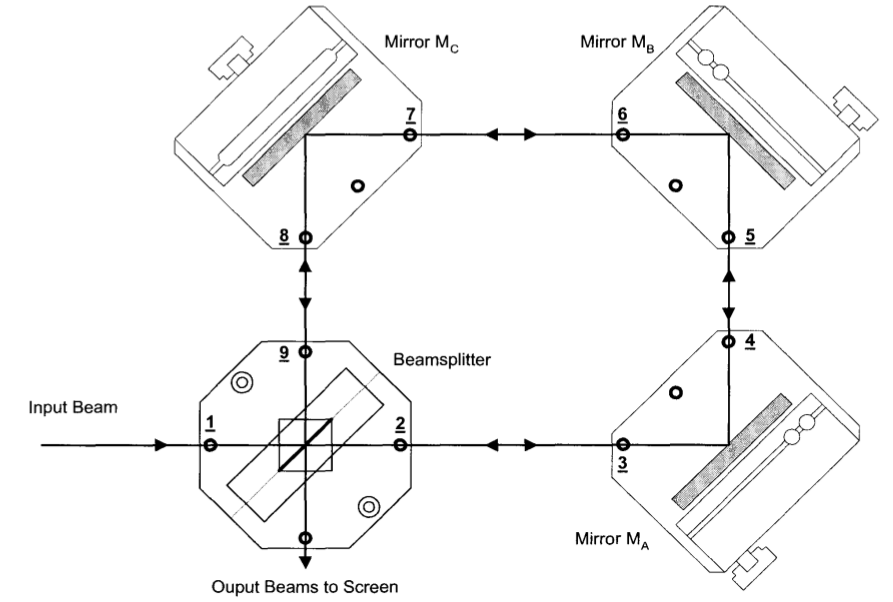
\includegraphics[width=0.5\textwidth]{Bild2.png}
  \caption{Der Strahlengang mit möglichen Positionen der Beam-Paddles \cite{anleitung}.}
  \label{fig:2}
\end{figure}
\noindent
Nach der Justage wird zunächst eine Messung zur Maximierung des Kontrastes durchgeführt.
Dazu wird der Doppelglashalter im Strahlengang platziert und der Winkel des
Polarisationsfilters zwischen $\SI{0}{\degree}$ und $\SI{90}{\degree}$ variiert
(zwischen $\SI{0}{\degree}$ und $\SI{30}{\degree}$ und zwischen $\SI{60}{\degree}$
und $\SI{90}{\degree}$ in 10er Schritten, zwischen $\SI{30}{\degree}$ und
$\SI{60}{\degree}$ in 5er Schritten). Dabei wird jeweils die minimale und maximale Diodenspannung
(bei Auslöschung und Verstärkung) gemessen, welche an einem Oszilloskop angezeigt wird.

\subsection{Bestimmung der Brechungsindizes}
\label{sub:brechindizes}
Für die Bestimmung der Brechungsindizes von Glas und Luft wird eine Zählapparatur
verwendet, die die Nulldurchgänge der fallenden Flanke der Diodenspannung zählt.
Der Winkel des Doppelglashalters wird nun in einem Bereich von $\SI{10}{\degree}$
bei konstanter langsamer Geschwindigkeit variiert. Anschließend wird die Anzahl,
der Nulldurchgänge und damit die Anzahl der Maxima abgelesen.
Diese Messung wird fünf mal durchgeführt.
Anschließend wird der Doppelglashalter aus dem Strahlengang entfernt und stattdessen
eine Gaszelle in dem Strahlengang eines Strahls platziert, in welcher über einen
Kompressor ein möglichst gutes Vakuum erzeugt werden kann. Anschließend wird
wieder über Ventile langsam Luft in die Gaszelle gelassen und dabei die Anzahl
der Nulldurchgänge gezählt, die bis zum vollständigen Druckausgleich auftreten.
Diese Messung wird drei mal durchgeführt.

\section{Auswertung}
\label{sec:auswertung}

\subsection{Fehlerrechnung}
\label{sec:fehlerrechnung}
Für die Fehlerrechnung sowie den mathematischen Teil der Auswertung wird auf
  $\textsc{Python}$ \cite{python} zurückgegriffen:\\
Die in der Auswertung verwendeten Mittelwerte mehrfach gemessener Größen sind
gemäß der Gleichung
\begin{equation}
    \bar{x}=\frac{1}{n}\sum_{i=1}^n x_i.
    \label{eq:mittelwert}
\end{equation}
\noindent
bestimmt. Dieser ist implementiert durch die Funktion $\textsc{mean}$ aus dem Paket
  $\textsc{Numpy}$ \cite{numpy}. Die Standardabweichung des Mittelwertes ergibt sich dabei zu

\begin{equation}
    \mathup{\Delta}\bar{x}=\sqrt{\frac{1}{n(n-1)}\sum_{i=1}^n\left(x_i-\bar{x}\right)^2}.
    \label{eq:standardabweichung}
\end{equation}
\noindent
Dieser wird durch die
$\textsc{scipy.stats}$ \cite{scipy} Funktion $\textsc{sem}$ berechnet.\\
Fehlerfortpflanzung wird
durch die Bibliothek $\textsc{uncertainties}$ \cite{uncertainties} automatisiert.
Regressionen sowie deren Fehler wurden durch die $\textsc{Numpy}$
Funktion $\textsc{curve-fit}$ berechnet.
Grafiken wurden mit $\textsc{matplotlib}$ \cite{matplotlib}
erstellt.
\subsection{Kontrastmessung}
Um den Kontrast zu bestimmen werden an einer Photodiode abfallende
Minimal- und Maximalspannungen für verschiedene Polarisatorstellungen
$\theta_{\symup{P}}$ gemessen. Die gemessenen
Werte und die damit errechneten Kontrastwerte nach Formel \eqref{eqn:kontrast} sind in Tabelle \ref{A_tab:1}
zu sehen.
Der Kontrast, der abhängig von eingestellten Winkel ist, wird nach Formel
\eqref{eqn:kontrastwinkel} mit einer Funktion
\begin{equation}
  K(\theta_{\symup{P}}) = |{\alpha \sin{(\beta \theta_{\symup{P}}+\gamma)}}| + \delta
  \label{A_eqn:1}
\end{equation}
gefittet. Dabei ergeben sich die Parameter:
\begin{align}
\begin{split}
  \alpha &= \num{0.758(3)}\\
  \beta &= \num{1.916(35)}\\
  \gamma &= \SI{-0.087(31)}{\degree} \\
  \delta &= \num{0.007(25)}
\end{split}
\label{A_eqn:2}
\end{align}
Der dazugehörige Fit ist in Abbildung \ref{A_abb:1} dargestellt.
\begin{table}[H]
  \centering
  \caption{Die Mess- und Kontrastwerte $K$.}
  \label{A_tab:1}
  \begin{tabular}{c c c c}
    \toprule
    $\theta_{\symup{P}}$ / \si{\degree} & $I_{\symup{max}}$ / \si{\volt} &
    $I_{\symup{min}}$ / \si{\volt} & $K$\\
    \midrule
    0 & -4.31 & -3.72 & 0.07 \\
    10 & -3.62 & -2.31 & 0.22 \\
    20 & -3.22 & -1.28 & 0.43 \\
    30 & -2.94 & -0.72 & 0.61 \\
    35 & -2.92 & -0.67 & 0.63 \\
    40 & -3.08 & -0.53 & 0.70 \\
    45 & -3.23 & -0.47 & 0.75 \\
    50 & -3.56 & -0.41 & 0.80 \\
    55 & -3.88 & -0.50 & 0.77 \\
    60 & -4.28 & -0.75 & 0.70 \\
    70 & -5.03 & -1.06 & 0.65 \\
    80 & -5.25 & -2.19 & 0.41 \\
    90 & -4.84 & -3.72 & 0.13 \\
    \bottomrule
  \end{tabular}
\end{table}
\begin{figure}[H]
  \centering
  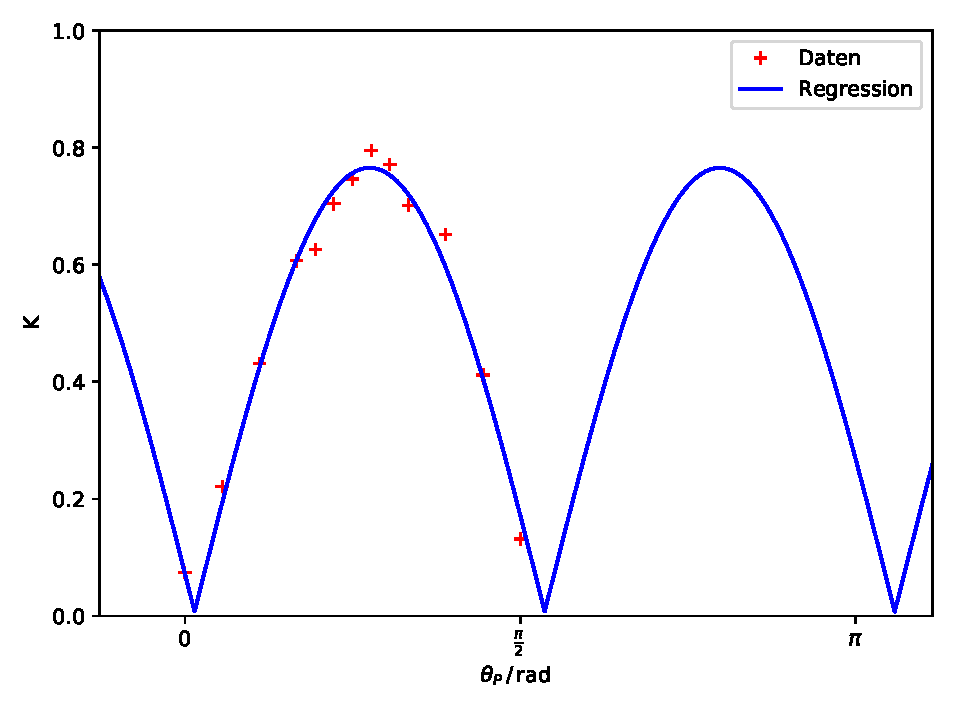
\includegraphics[width=0.7\textwidth]{Kontrast.pdf}
  \caption{Der Kontrast $K$ des Interferometers in Abhängigkeit von der Polarisatorstellung
  $\theta_{\symup{P}}$ mit einer Regression.}
  \label{A_abb:1}
\end{figure}
\noindent
Um den Kontrast optimal unteruschen zu können, wird das Maximum der
Kontrastfunktion \eqref{A_eqn:1} gesucht. Dafür nutzt man die Ableitung
und es ergibt sich die notwengdige Bedingung:
\begin{equation*}
  \frac{dK(\theta_{\symup{P}})}{d\theta_{\symup{P}}} = \alpha \beta \cos{
  (\beta \theta_{\symup{P}} + \gamma)} \stackrel{!}{=} 0.
\end{equation*}
Mit Hilfe von
\begin{equation*}
  \beta \theta_{\symup{P, max}} + \gamma = \frac{\pi}{2} \; \leftrightarrow \;
  \theta_{\symup{P, max}} = \frac{\frac{\pi}{2} - \gamma}{\beta}
\end{equation*}
folgt, mit Hilfe der Fitparameter aus \eqref{A_eqn:2} ein Wert von
\begin{equation*}
  \theta_{\symup{P, max}} = \SI{49.6(13)}{\degree}.
\end{equation*}
Die folgenden Messungen wurden bei dieser Polarisatorstellung durchgeführt.

\subsection{Brechungsindex von Glas}
Die Glasplättchen sind in einem relativen Winkel $\Theta = 2 \theta_0 = 2 \cdot \SI{10}{\degree}$
zueinander angeordnet. Zusammen mit der Plättchendicke von $\mathup{T}=\SI{1}{\milli\metre}$
sowie einer Laserwellenlänge von \SI{633}{\nano\metre} in Formel \eqref{A_eqn:3}
eingesetzt ergeben sich aus den Messdaten die Werte, welche in Tabelle \ref{A_tab:2}
stehen, wobei $\theta_0 = \SI{10}{\degree}$ gilt. Es wurden 5 Messreihen
aufgenommen. Mittelung über die Messwerte aller Messreihen liefert einen Wert von:
\begin{equation*}
  n_{\symup{Glas}} = \num{1.561(12)}.
\end{equation*}

\begin{table}[h!]
  \centering
  \caption{Messwerte mit Brechungsindizes der 5 Messreihen. Es wurde ein
  Intervall von \SI{10}{\degree} abgefahren.}
  \label{A_tab:2}
  \begin{tabular}{c | c}
    \toprule
    $M$ & $n$ \\
    \midrule
    34 & 1.60 \\
    34 & 1.55 \\
    35 & 1.57 \\
    35 & 1.57 \\
    35 & 1.52 \\
    \bottomrule
  \end{tabular}
\end{table}
\subsection{Brechungsindex von Luft}
Messwerte und nach Formel \eqref{eqn:brechgas} bestimmte Brechungsindizes sind in Tabelle
\ref{A_tab:3} dargestellt. Alle Interferezstreifenmessungen wurden mit einem Fehler
von $\pm \, 2$ versehen, da es bei der Rückkehr auf Umgebungsdruck in der Gaszelle
zu Fehlzählungen kommt. Die Länge der Zelle beläuft sich auf $\mathup{L} = \SI{10}{\centi\metre}$.
Wieder beträgt die Laserwellenlänge \SI{633}{\nano\metre}.\\
Es ergibt sich also ein Wert von
\begin{equation*}
  n_{\symup{Luft}} = \num{1.000268(13)}.
\end{equation*}

\begin{table}[h!]
  \centering
  \caption{Gezählte Interferenzstreifen $\mathup{N}$ mit berechneten
  Brechungsindizes für Luft und Mittelwert $\overline{n}$.}
  \label{A_tab:3}
  \begin{tabular}{c c c}
    \toprule
    & $\mathup{N}$ & $n$ \\
    \midrule
    & 43 $\pm$ 2 & \num{1.000272(13)} \\
    & 42 $\pm$ 2 & \num{1.000266(13)} \\
    & 42 $\pm$ 2 & \num{1.000266(13)} \\
    \midrule
    $\overline{n}$ & & \num{1.000268(13)}\\
    \bottomrule
  \end{tabular}
\end{table}

\section{Diskussion}
\begin{table}[h!]
  \centering
  \caption{Übersicht über die Messergebnisse mit Literaturwerten.}
  \label{D_tab:1}
  \begin{tabular}{c c c}
    \toprule
    & Messung & Literatur \\
    \midrule
    $n_{\symup{Glas}}$ & \num{1.561(12)} & \num{1.5} \cite[S. 11-5]{anleitung}  \\
    $n_{\symup{Luft, \SI{633}{\nano\metre}}}$ & \num{1.000268(13)} & \num{1.000277} \cite{Luft} \\
    \bottomrule
  \end{tabular}
\end{table}
\noindent
Tabelle \ref{D_tab:1} beinhaltet die gemessenen und die Literaturwerte. Es zeigt sich, dass
der Literaturwert für die Luftmessung in der Messungenauigkeit liegt.
Der in dem Versuch errechnete Wert für die Glasmessunghat allerdings nur eine
sehr kleine Abweichung zum Literaturwert. Das könnte eventuell an dem verwendeten
Glas liegen. Dies könnte eine andere Zusammensetzung haben, als das, das für den Literaturwert
genutzt wurde.
Bei der Messung des Brechnungsindex' von Luft konnte das Fehlerintervall nur getroffen
werden, da die Interfernzstreifenzählung nicht als fehlerfrei angesehen werden konnte
und ein pauschaler Fehler von $\pm \,\, 2$ angenommen wurde.
Es konnte außerdem beobachet werden, dass manchmal die Interferenzstreifen
von der Ausleseelektronik nicht aufgenommen werden konnten, da der Druck in der
Gaszelle etwas zu rasant anstieg. Daher ist hier ein systematischer
Fehler nicht auszuschließen. Dennoch ist der errechnete Wert ziemlich präzise am
Literaturwert.\\
Als weitere Fehlerquelle ergibt sich auch die Justage des Interferometers.
Bei der Kontrastfunktion zeigt sich eine relativ eindeutige $\frac{\pi}{2}$-Periode
und auch das Maximum ist in dem zu erwarteten Bereich. Allerdings sind auch
Fehler sichtbar, die durch eine bessere Justage verbessert werden könnten.
Dadurch würde sich ein besserer Kontrastwert ergeben und damit wäre das Auflösungsvermögen
des Interferometers besser.


\newpage
\nocite{*}
\printbibliography
\end{document}
